\section{Multigrid}
In this section, we will test the coarse part of the preconditioner : the multigrid solver. This will be done in two steps. First, we will verify a well known property of the multigrid solvers : the h-independent convergence. We will also compare the number and iterations needed while varying key parameters of the model. Those tests will be performed on various meshes. The second part will focus on the influence of hanging nodes on the numerical solution. 

Let us before all present a type of numerical solution that can be obtained using the multigrid solver. Figure \ref{multi_simple_sol} shows an example of the numerical solution computed. We can see that even with $p=1$, we have a good approximation. This is because the forcing term is not at all oscillatory.

\begin{figure}
\centering
\includegraphics[scale=0.35]{Results/multi_simple_sol.eps}
\caption{Numerical solution using the multigrid solver of $\nabla^2 u = f$ for $f = -2\tanh(3x)\tanh(3y)(18-9\tanh^2(3x)-9\tanh^2(3y))$}
\label{multi_simple_sol}
\end{figure}

\subsection{H-independent convergence}
Let us first verify that our geometric multigrid solver has the required property and that the same number of iterations is needed to obtain a given accuracy, however small the elements. We will use the model problem throughout this section with the same right hand side. For all the tests below, the domain  will be : $\Omega = [-1;1]^2$. We will solve : 

\begin{align}
\nabla^2 u &= -\frac{\pi^2}{2}cos(\frac{\pi}{2}x)cos(\frac{\pi}{2}y) &\text{on $\Omega$} \\
u &= 0  &\text{on $\Gamma$}
\end{align}

It is easy to see that for the given domain, we have an analytic solution : 
$$u(x,y) = cos(\frac{\pi}{2}x)cos(\frac{\pi}{2}y))$$ 


Let us now explain how we define the error. We will look at the absolute difference between the value of the approximation and the value of the analytic solution at the global nodes and take the maximum. Formally, we have that the error after iteration $k$, $e_k$ is :

$$e_k = \max_i |u(x_i,y_i) - u_i^k|$$

Where $u_i^k$ is the value of our approximation at the global node $i$ after iteration $k$. Since $u_i^0 = 0$ for all $i$, it is clear that $e_0 = 1$.

Figure \ref{multi_mesh} shows the two "supra meshes" that we will refine during the tests. Some refinements will be uniform and some will be so that we have the presence of hanging nodes. We can note that even for the crooked mesh, the elements are not really distorted. It does not matter since we are only testing the h-independent convergence. Having a mesh with elements that are more distorted will only influence the accuracy of the approximation and not how the algorithm solve the linear system we want to solve. 

\begin{figure}
\centering
\begin{subfigure}{.5\textwidth}
  \centering
  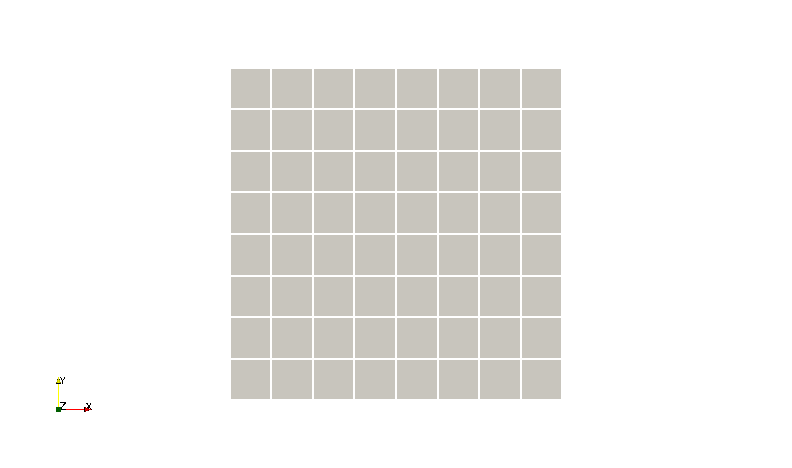
\includegraphics[width=1.2\linewidth]{Results/multi_mesh_1.png}
  \caption{Regular mesh}
  \label{multi_mesh_1}
\end{subfigure}%
\begin{subfigure}{.5\textwidth}
  \centering
  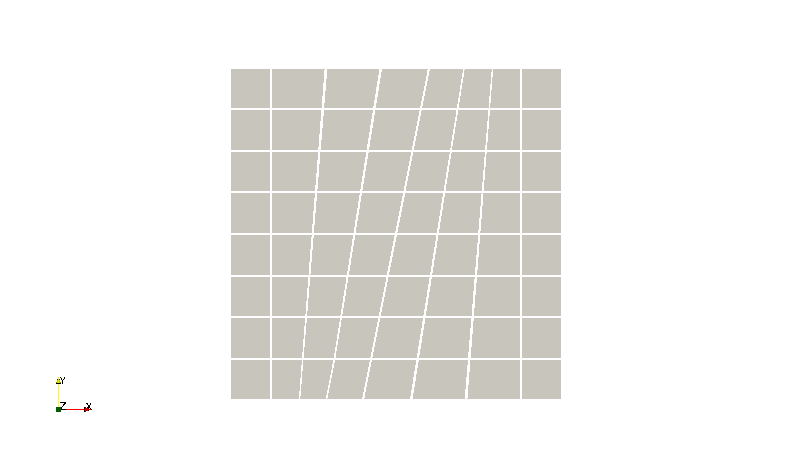
\includegraphics[width=1.2\linewidth]{Results/multi_mesh_2.png}
  \caption{Crooked mesh}
  \label{multi_mesh_2}
\end{subfigure}
\caption{The two "supra meshes" that will be refined during the tests for the multigrid solver. We have one regular mesh (left) where the elements are squares and one crooked mesh (right) where the elements are slightly distorted.}
\label{multi_mesh}
\end{figure}



Let us start with a simple V-cycle on the regular mesh (figure \ref{multi_mesh_1}) that we will refine uniformly. We will compare the errors when we increase the number of degrees of freedom and for different $\nu_1$ and $\nu_2$. The sum of the two smoothing parameters is chosen to be constant so that we have the same number of Jacobi iterations for all pairs $\nu_1$ and $\nu_2$. Here, we chose the sum to be equal to four.


\begin{table}
\centering
\begin{tabular}{c|ccccc}
\hline
 N & $2.6\:10^5$ & $1.1\:10^6$ & $4.2\: 10^6$& $1.7\:10^7$ & $6.7\:10^7$ \\
 \hline
  & $\nu_1=2$ & $\nu_2=2$ & & &\\
  \hline
  $e_1$ & 3.56e-02 & 3.56e-02 & 3.56e-02 & 3.56e-02 & 3.56e-02\\
  $e_2$ & 1.34e-03 &	1.34e-03 &	1.34e-03	& 1.34e-03	& 1.34e-03\\
  $e_3$ & 5.42e-05 &	5.66e-05 &	5.72e-05 &	5.73e-05 &	5.73e-05\\
  $e_4$ & 3.11e-06 &	2.90e-06 &	3.45e-06 &	3.59e-06 &	3.62e-06\\
  $e_5$ & 3.30e-06 &	9.48e-07 &	3.62e-07	& 3.50e-07 &	3.85e-07\\
  $e_6$ & 3.17e-06 &	8.14e-07 &	2.26e-07 &	8.26e-08 &	5.23e-08\\
  \hline
  & $\nu_1=3$ & $\nu_2=1$ & & &\\
  \hline
  $e_1$ & 3.70e-02 &	3.71e-02 &	3.71e-02 &	3.71e-02 &	3.71e-02\\
  $e_2$ & 1.62e-03 &	1.63e-03 &	1.63e-03 &	1.63e-03 &	1.63e-03\\
  $e_3$ & 1.04e-04 &	1.06e-04 &	1.07e-04 &	1.07e-04	& 1.07e-04\\
  $e_4$ & 1.10e-05 &	1.22e-05 &	1.27e-05 &	1.29e-05 & 	1.29e-05\\
  $e_5$ & 4.47e-06 &	2.20e-06 &	1.96e-06 &	2.10e-06 & 	2.13e-06\\
  $e_6$ & 3.34e-06 &	1.00e-06 &	4.38e-07 &	3.53e-07 &	3.88e-07\\
  \hline
  & $\nu_1=1$ & $\nu_2=3$ & & &\\
  \hline
  $e_1$ & 3.57e-02 &	3.57e-02 &	3.57e-02 &	3.57e-02 &	3.57e-02\\
  $e_2$ & 1.29e-03 &	1.29e-03 &	1.29e-03 &	1.29e-03 &	1.29e-03\\
  $e_3$ & 4.66e-05 &	4.89e-05 &	4.95e-05 &	4.96e-05 &	4.97e-05\\
  $e_4$ & 1.53e-06 &	1.53e-06 &	2.10e-06 &	2.24e-06 &	2.28e-06\\
  $e_5$ & 3.08e-06 &	7.31e-07 &	1.43e-07 &	1.17e-07 &	1.51e-07\\
  $e_6$ & 3.14e-06 &	7.83e-07 &	1.95e-07 &	4.80e-08 &	1.13e-08\\
  \hline
   & $\nu_1=4$ & $\nu_2=0$ & & &\\
  \hline
  $e_1$ & 4.55e-02 &	4.55e-02 &	4.55e-02 &	4.55e-02 &	4.55e-02\\
  $e_2$ & 3.26e-03 &	3.26e-03 &	3.26e-03 &	3.26e-03 &	3.26e-03\\
  $e_3$ & 4.64e-04 &	4.71e-04 &	4.71e-04 &	4.71e-04 &	4.71e-04\\
  $e_4$ & 9.24e-05 &	9.60e-05 &	9.65e-05 &	9.67e-05 &	9.67e-05\\
  $e_5$ & 1.74e-05 &	2.04e-05 &	2.12e-05 &	2.14e-05 &	2.14e-05\\
  $e_6$ & 6.17e-06 &	3.86e-06	& 4.55e-06	& 4.74e-06 &	4.78e-06\\
  \hline
  & $\nu_1=0$ & $\nu_2=4$ & & &\\
  \hline
  $e_1$ & 3.58e-02 &	3.58e-02 &	3.58e-02 &	3.58e-02 &	3.58e-02\\
  $e_2$ & 1.29e-03 &	1.29e-03 &	1.29e-03 &	1.29e-03 &	1.29e-03\\
  $e_3$ & 4.53e-05 &	4.77e-05 &	4.82e-05 &	4.84e-05 &	4.84e-05\\
  $e_4$ & 1.17e-06 &	1.31e-06 &	1.89e-06 &	2.03e-06 &	2.07e-06\\
  $e_5$ & 3.03e-06 &	6.80e-07 &	9.14e-08 &	7.66e-08 &	1.12e-07\\
  $e_6$ & 3.13e-06 &	7.76e-07 &	1.87e-07 &	4.04e-08 &	3.62e-09\\
  \hline
\end{tabular}
\caption{Errors after $k$ iterations of a V-cycle ($e_k$) for the regular mesh uniformly refined to have $N$ degrees of freedom and for different values of the parameters $\nu_1$ and $\nu_2$}
\label{multi_err_nu}
\end{table}

The results are shown in table \ref{multi_err_nu}. We can see that we indeed have an h-independent convergence of the solver. For every pair of the smoothing parameters, at least for the first few iterations, the error $e_k$ is identical for all values of $N$. Except for the pair $\nu_1 = 4$ and $\nu_2 = 0$, each iteration roughly decrease the error by one decimal point.

We can also note that the values of the parameters influence the convergence. For this particular problem and this particular mesh, the values $\nu_1 = 0$ and  $\nu_2 = 4$ seem to be the best as the error is smaller after the same number of iterations than for the other pairs. The less post smoothing iterations ($\nu_2$) we do, the slower the convergence. This is true for $\nu_2 = 1$ where the error on the finest mesh after six iterations is a hundred times larger than on the same mesh after the same number of iterations for $\nu_2=4$, and it is clearer still for $\nu_2=0$ where the error is a thousand times larger after six iterations on the finest mesh.

We have to note that even tough the errors are identical for all meshes at first, we have a difference after a few iterations. This can be explained by the fact that our geometric multigrid algorithm actually solves a linear system whereas the error is measured as the difference between the analytic solution and the solution of the linear system. Thus, even if we solved the linear system exactly, we would still have an error and that error should decrease as the number of degrees of freedom increases. This is indeed what we observe here. For example, for the mesh with $N=2.6\:10^5$, we can see that after six iterations, we have almost converged and that the error stays around $3.14\:10^{-6}$. Even if we did several more iterations, the error would not decrease significantly. That is because we have the solution of the linear system and the error is only due to the discretization. If we refine the mesh and go to $N=6.7\:10^7$, then we can get smaller errors (of the order of $10^{-8}$).

Let us now explore the results for the crooked mesh (figure \ref{multi_mesh_2}). Here also, we should expect an h-independent convergence. We only show the results for $\nu_1=2$ and $\nu_2=2$ but the same commentary applies for the other pairs. The results can be seen on table \ref{multi_err_crook}

\begin{table}
\centering
\begin{tabular}{c|ccccc}
\hline
N & $2.6\:10^5$ & $1.1\:10^6$ & $4.2\: 10^6$& $1.7\:10^7$ & $6.7\:10^7$ \\
 \hline
  & $\nu_1=2$ & $\nu_2=2$ & & &\\
  \hline
  $e_1$ & 3.64e-02 &	3.64e-02 &	3.64e-02 &	3.64e-02 &	3.64e-02\\
  $e_2$ & 2.56e-03 &	2.49e-03 &	2.46e-03	& 2.44e-03 &	2.43e-03\\
  $e_3$ & 7.41e-04 &	6.33e-04 &	5.80e-04 &	5.54e-04 &	5.41e-04\\
  $e_4$ & 6.15e-04 &	3.15e-04 &	1.62e-04 &	1.35e-04 &	1.28e-04\\
  $e_5$ & 5.96e-04 &	3.01e-04 &	1.52e-04 &	7.67e-05	& 4.76e-05\\
  $e_6$ & 5.91e-04 &	2.98e-04 &	1.50e-04 &	7.50e-05 &	3.77e-05\\
  \hline
\end{tabular}
\caption{Errors after $k$ iterations of a V-cycle ($e_k$) for the crooked mesh uniformly refined to have $N$ degrees of freedom and for $\nu_1=2$ and $\nu_2=2$}
\label{multi_err_crook}
\end{table}

We can see that the for the first few iterations, the error $e_k$ is independent of the mesh. However, the note we made earlier is much clearer here. Because the mesh is not regular, the effect of discretization are more important and therefore we will not reach the same accuracy than we did before. That is why after six iterations, the less refined grid ($N = 2.6\:10^5$) still has an error of $5.91\:10^{-4}$. More iterations will not have a great impact on the solution since the error is mostly due to the discretization.

\subsection{Influence of hanging nodes}
We will now investigate the influence of hanging nodes on our solution. We will present the results only for the regular mesh but the tests have been performed on both and the same conclusions apply to the crooked mesh.

We will compare the values of the error between one mesh with no hanging nodes, one where we only have refined the lower left part of the domain once, and one where we have a rapid transition between two parts  of different refinement level (which will occur often in AMR).

Figure \ref{multi_mesh_hanging} presents the latter two meshes. For the mesh in figure \ref{multi_mesh_hanging_2}, we have refined thrice more in a certain region than in the adjacent one. Since we do not allow adjacent quadrants to be more than one level apart, we obtain a "layer" where the levels of the quadrants is rapidly changing. In order to compare solutions, we made sure that the largest quadrants in all three meshes had the same size. This means that the meshes with hanging nodes have a lot more degrees of freedom.  

\begin{figure}
\centering
\begin{subfigure}{.5\textwidth}
  \centering
  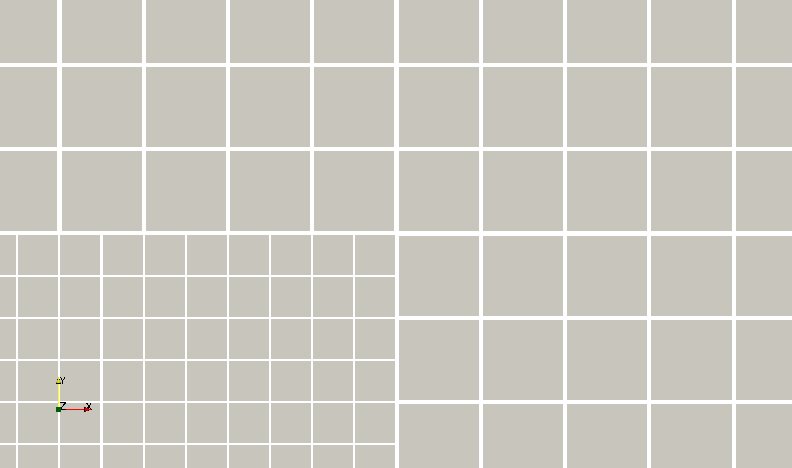
\includegraphics[width=0.8\linewidth]{Results/multi_mesh_hanging_1.png}
  \caption{Two levels}
  \label{multi_mesh_hanging_1}
\end{subfigure}%
\begin{subfigure}{.5\textwidth}
  \centering
  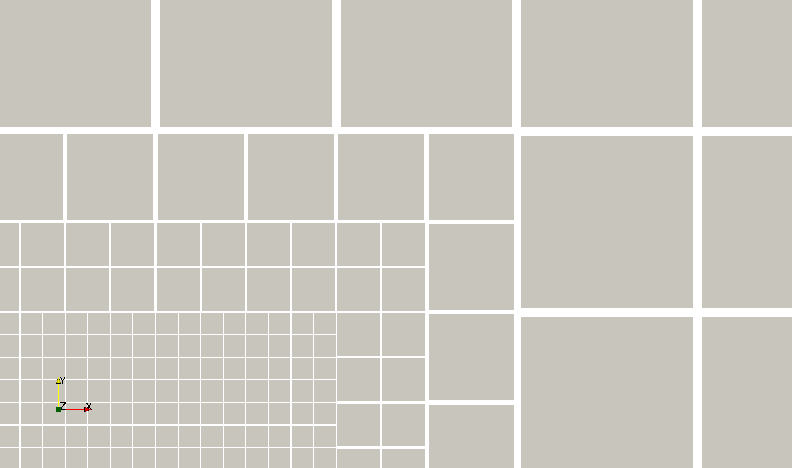
\includegraphics[width=0.8\linewidth]{Results/multi_mesh_hanging_2.png}
  \caption{Levels rapidly changing}
  \label{multi_mesh_hanging_2}
\end{subfigure}
\caption{Zoom on a certain part of the two meshes containing hanging nodes that will be used to test the multigrid solver. We have one mesh where we only have refined a part of the domain once more than the rest (left) and a mesh where we have refined a part thrice more than the rest which results in levels changing rapidly (right).}
\label{multi_mesh_hanging}
\end{figure}


\begin{table}
\centering
\begin{tabular}{c|ccc}
\hline
Meshes & No hanging nodes & Figure \ref{multi_mesh_hanging_1} & Figure \ref{multi_mesh_hanging_2}\\
\hline
N & $4.2\:10^6$ & $7.3\:10^6$ & $7.0\: 10^7$ \\
  \hline
  $e_1$ & 3.56e-02 &	3.56e-02 &	3.56e-02 \\
  $e_2$ & 1.34e-03 &	1.34e-03 &	1.34e-03	\\
  $e_3$ & 5.72e-05 &	5.72e-05 &	5.74e-05 \\
  $e_4$ & 3.45e-06 &	3.47e-06 &	3.64e-06 \\
  \hline
\end{tabular}
\caption{Errors after $k$ iterations of a V-cycle ($e_k$) for a mesh without hanging nodes and the two meshes presented in figure \ref{multi_mesh_hanging}. Each mesh has $N$ degrees of freedom and the smoothing parameters were $\nu_1 = 2$ and $\nu_2 =2$.}
\label{multi_err_hanging}
\end{table}

Table \ref{multi_err_hanging} shows the results for the three different meshes using a V-cycle and with the smoothing parameters  $\nu_1=2$ and $\nu_2 = 2$. Here again, we can see that the convergence is h-independent and that one iteration gives us roughly one more decimal. The presence of hanging nodes has no influence on the error we observe after a given number of iterations. The same result is observed with all pairs of the smoothing parameters and with other meshes.

This will be important in the next sections when we will use our multigrid solver as a preconditioner. Indeed, we will see that it is the coarse correction that allow for h-independent convergence.  


 



